\section{Description of the Model and Implementation}

\subsection{Description of the main function}

In our model one can compare roundabouts with crossroads, controlled by traffic lights. One can use an arbitrary combination of roundabouts and crosslights in a $N \times M$ map.\\Main input of the simulation are car and pedestrian densities, which can be entered as arrays. The simulation can be done with different probabilities for the car to go straight ahead. Cars turning left or right will have the same probability. The simulation will generate a plot over these densities as x- and y- axis and the average flow and average speed as z-axis in different colors. 

\begin{center} 
$flow = density \cdot speed$
\end{center}

\subsubsection{Implementation}

We have created a big matrix to display the simulation, containig all roads and intersections. Cars will be painted in blue and pedestrians in yellow. To the right of lanes heading towards a crossroad and to the left of lanes for cars turning left are traffic light cells, which are red or green. Next to the lanes leaving is a traffic light too, but for pedestrians. Many matrices more are needed to store status informations that can change. So for most following matrices, there are two versions, representing current and next status. After every iteration status next will assigned to current. 

\subsection{crossroad}
Depending on the pedestrian density, there are three different signalisation modes. For densities smaller than 0.3, cars that turn can always be blocked currently by a pedestrian. If the density is between 0.3 and 0.6, they can only block cars turning left. And if the density is even higher there should be no conflicts between cars and pedestrians. But if the car densities are very high, it can happen that the fixed yellow phase for changing the signalisation is too short to let all the cars leave the crossroad.\\

A further input parameter in the main-function is the probability of a car driving straight ahead. Cars that turn left and right have the same probability. So depending on these probabilities the relative time for light phases are different. To get the absolute time of a phase, one has to multiply it with a constant, indicating how often you change the signalisation.\\

It would be efficient if cars leaving one intersection would just arrive at the next one in a �green�-phase, so that the crossroad could take advantage of the randomisation process when entering a roundabout. A clever solution for this interesting problem is left to a next group, hopefully. We just added a phase offset between two crossroads, defined by the average time a car needs to drive from one intersection to the next and the fixed street lengths.\\

In contrast to the simulation of Wood and B�cheler and to the roundabout, cars entering the crossroad can have speed bigger than one cell per iteration. So cars can drive straight ahead with maximal speed of 5 cells according to the Nagel-Schreckenberg model \cite{schreckenberg} . Cars turning left or right are limited to maximal 2 cells per iteration.\\

\subsubsection{Implementation}
A crossroad consists of three $6 \times 6$-Matrices, so that for every cell information about is there a car, its speed and direction can be stored. Furthermore two $4 \times 8$ -Matrix for 4 lanes of length 8 cells at every street heading towards the crossroad for cars turning left are needed to decide if there's a car and store its speed. For cars driving ahead or turning right one $4 \times 8$-Matrix indicates the direction. 

\subsection{Roundabout}
Our implementation of the roundabout consits of a circle with 12 cells and 4 roads, which lead towards it. Every street has pedestrian crossings in front of each roundabout. 
Like in the real world, cars inside the roundabout have priority over cars wanting to enter them and pedestrians have priority over cars at the pedestrian crossings, 
with the addition, that pedestrians will only walk on the road if there is no car staying or driving on the cell they wants to walk on. 
Inside the crossroad the speed a car can have is limited to 1 cell per iteration step. \\

A car which wants to leave the roundabout at the next exit will indicate, in our plot this is shown by giving these cars a darker colour. 
The exit a car will take is calculated from the probability ahead like in the crossroad, but with a fixed probability of 5 \% for a car which will take the 4th exit (i.e. the car will turn around). \\
\subsubsection{Implementation}
This is implemented with many arrays, three arrays for the circle, one which shows whether there is a car or not, and if the car wants to leave at the next exit. 
The second is used to store the velocity of the car and the third is used to store, how many exits the car will pass without leaving.\\

The entries and exits of the roundabout are randomly blocked by pedestrians. For this reason two 'buckets' are created, representing pedestrian islands between inwards and outgoing streets. If a pedestrian crosses an outgoing street, the bucket makes sure, that in the next iteration inwards street will be blocked. 


\subsection{Graphical implementation}

One very important part in simulating a specific problem is visualization. First for checking if a given implementation makes sense the way one has written it, for bug fixing and for adjusting the parameters of the model to the real world problem.

\subsubsection{Preparatory work}
Before programming something out of the head one has to create an idea of how a problem could be implemented. One has to be careful to not exaggerate the model and fix too much on unimportant details, but to keep the main ideas clear and simple. 

\begin{figure}[htb]
	\centering
		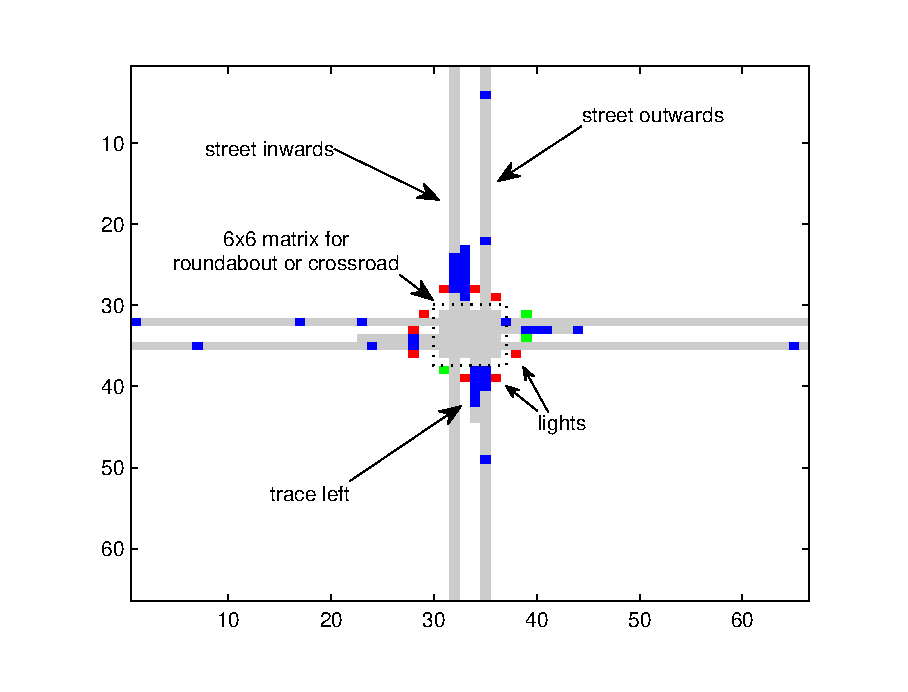
\includegraphics[width=0.8\textwidth]{images/description_mapping_overview.eps}
	\caption{Overview over the implementation of the plot.}
	\label{fig:description_mapping_overview}
\end{figure}

\autoref{fig:description_mapping_overview} shows how we finally ended in, because it shows the elementary cell of each intersection. Our model consisted of
\begin{itemize}
	\item a intersection (either roundabout or a crossroad)
	\item 8 streets for each direction of the crossroad (each with a out- and ingoing street)
	\item	pedestrians (not in the figure)
	\item	cars (in blue)
	\item	traffic lights for the cars and pedestrians in the case of a roundabout
	\item a trace for the cars that turn left in the case of a crossroad
\end{itemize}

In the following sections I will explain the programming details of this figure.

\subsubsection{Implementation}
For each type of intersections we have written a function that works out the paths of the cars and returns this information in a $6 \times 6$ matrix. Furthermore information about the pedestrians, the traffic light phases and the cars on the left trace are returned. I implemented these by creating a large matrix

\[
 \begin{split}
\mathrm{map} = (\mathrm{(No. \ of \ intersections \ in \ x \ direction)} \cdot (2 \cdot \mathrm{streetlength} + 6) \times \\ 
 \mathrm{(No. \ of \ intersections \ in \ y \ direction)} \cdot (2 \cdot \mathrm{streetlength} + 6))
\end{split}
\]

in which we wrote all elements listed up above for each time step, that we looked at. The elements of the maps were encoded in a color code from $0$ to $2$, i.e.
\begin{itemize}
	\item	Car = $0.6$
	\item	Red light = $1.6$
	\item	Pedestrian = $0.8$
\end{itemize}
that were written into this large matrix.
By plotting this matrix with
\begin{center}
\texttt{imagesc(map)}
\end{center}
and using a colormap we were able to create a relatively realistic model (see figure above).


\begin{figure}[htb]
	\centering
		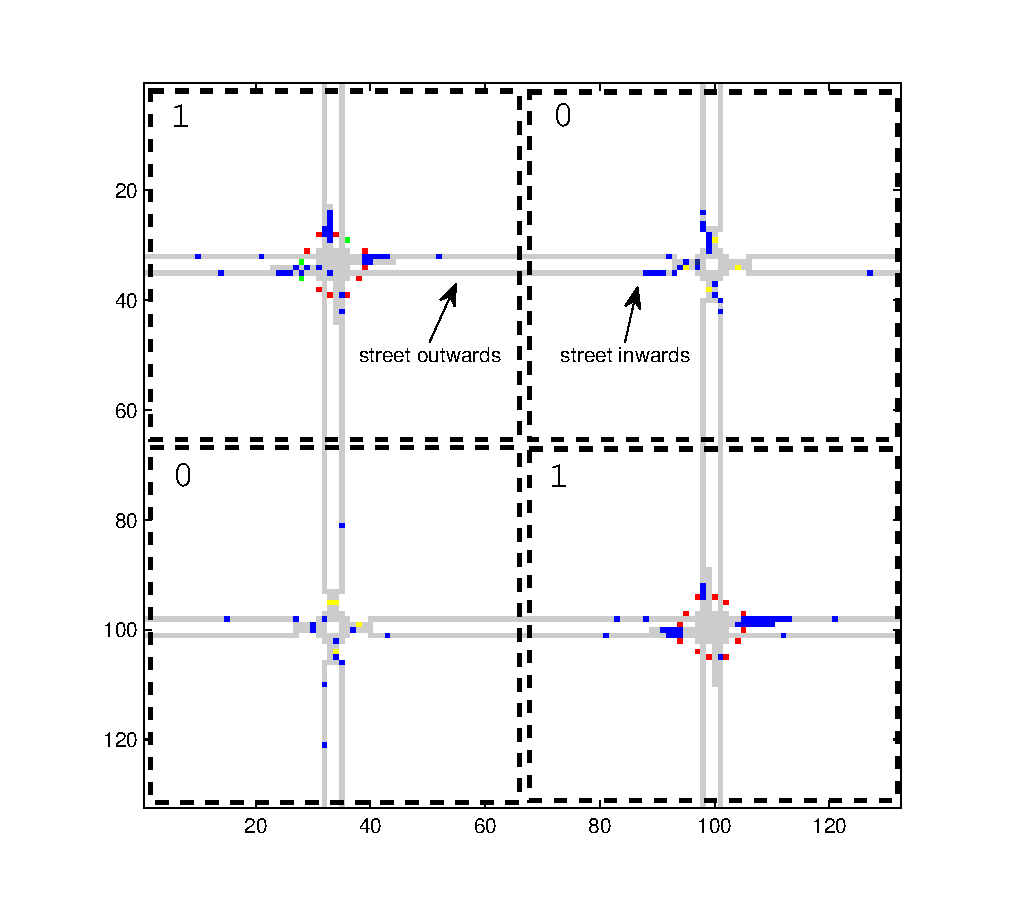
\includegraphics[width=0.8\textwidth]{images/description_mapping_detail.eps}
	\caption{Details about the implementation of the plot in the case of many intersections.}
	\label{fig:description_mapping_detail}
\end{figure}

We wanted to analyze how the traffic flow changes when we have many intersections in a map that are connected together to reproduce a more realistic view of the world. The configuration of each map was written into a matrix. This matrix had $0$ (corresponding to roundabout) and $1$ (corresponds to crossroad) as entries and corresponds to the rough structure of the map. Let's demonstrate this with \autoref{fig:description_mapping_detail}. We see in the top left and bottom right corners two crossroad and in the top right and bottom left corner two roundabouts. Naturally this would be denoted in a matrix as
\[
	\left(\begin{matrix}
1 & 0\\ 
0 & 1
\end{matrix}\right)
\]
and this is how we implemented it. Then the outgoing streets of the one cell are connected to the inwards streets of the neighboring cell and programing this, this results in these dynamic maps.

Furthermore we added the support of saving a video output of the this specific configuration. For further details see the code in the listings (see \autoref{plot_map}).

\newpage